\section{Date: 2026-10-30}
\noindent \textbf{Series ID: PUA0T17FL12073A647NCEN} 

\noindent This series is titled Poverty Universe, Age 0-17 for Leon County, FL and has a frequency of Annual. The units are Persons and the seasonal adjustment is Not Seasonally Adjusted.The observation start date is 1998-01-01 and the observation end date is 2024-01-01.The popularity of this series is 1. \\ 

\noindent \textbf{Series ID: SFXRHTSA} 

\noindent This series is titled Home Price Index (High Tier) for San Francisco, California and has a frequency of Monthly. The units are Index Jan 2000=100 and the seasonal adjustment is Seasonally Adjusted.The observation start date is 1987-01-01 and the observation end date is 2026-08-01.The popularity of this series is 9. \\ 

\subsection{Raw Regression}
\noindent Regresses the two series against each other directly. A significant result here can come just as easily from both series sharing a long-run trend as from any real relationship.

\begin{center}
\begin{tabular}{lclc}
\toprule
\textbf{Dep. Variable:}                      & value\_fred\_SFXRHTSA & \textbf{  R-squared:         } &     0.417   \\
\textbf{Model:}                              &          OLS          & \textbf{  Adj. R-squared:    } &     0.394   \\
\textbf{Method:}                             &     Least Squares     & \textbf{  F-statistic:       } &     17.87   \\
\textbf{Date:}                               &    Fri, 30 Oct 2026   & \textbf{  Prob (F-statistic):} &  0.000276   \\
\textbf{Time:}                               &        17:18:43       & \textbf{  Log-Likelihood:    } &   -147.30   \\
\textbf{No. Observations:}                   &             27        & \textbf{  AIC:               } &     298.6   \\
\textbf{Df Residuals:}                       &             25        & \textbf{  BIC:               } &     301.2   \\
\textbf{Df Model:}                           &              1        & \textbf{                     } &             \\
\textbf{Covariance Type:}                    &       nonrobust       & \textbf{                     } &             \\
\bottomrule
\end{tabular}
\begin{tabular}{lcccccc}
                                             & \textbf{coef} & \textbf{std err} & \textbf{t} & \textbf{P$> |$t$|$} & \textbf{[0.025} & \textbf{0.975]}  \\
\midrule
\textbf{const}                               &   -2231.4439  &      573.331     &    -3.892  &         0.001        &    -3412.242    &    -1050.646     \\
\textbf{value\_fred\_PUA0T17FL12073A647NCEN} &       0.0460  &        0.011     &     4.228  &         0.000        &        0.024    &        0.068     \\
\bottomrule
\end{tabular}
\begin{tabular}{lclc}
\textbf{Omnibus:}       &  2.121 & \textbf{  Durbin-Watson:     } &    0.831  \\
\textbf{Prob(Omnibus):} &  0.346 & \textbf{  Jarque-Bera (JB):  } &    0.876  \\
\textbf{Skew:}          &  0.111 & \textbf{  Prob(JB):          } &    0.645  \\
\textbf{Kurtosis:}      &  3.854 & \textbf{  Cond. No.          } & 2.67e+06  \\
\bottomrule
\end{tabular}
%\caption{OLS Regression Results}
\end{center}

Notes: \newline
 [1] Standard Errors assume that the covariance matrix of the errors is correctly specified. \newline
 [2] The condition number is large, 2.67e+06. This might indicate that there are \newline
 strong multicollinearity or other numerical problems.

\begin{figure}
\centering
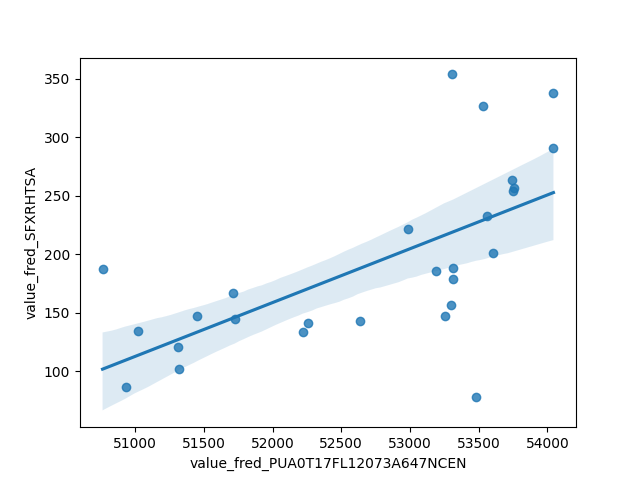
\includegraphics[scale = 0.9]{plots/plot_2026-10-30.png}
\caption{Raw Regression Plot for 2026-10-30}
\end{figure}
\newpage
\subsection{Detrended Regression}
\noindent Regresses the residuals of each series after removing its own linear time trend, so a shared trend can no longer drive the result on its own. A relationship that stays significant here is better evidence of a genuine link between the two series.

\begin{center}
\begin{tabular}{lclc}
\toprule
\textbf{Dep. Variable:}                                 & value\_fred\_SFXRHTSA\_detrended & \textbf{  R-squared:         } &     0.006   \\
\textbf{Model:}                                         &               OLS                & \textbf{  Adj. R-squared:    } &    -0.034   \\
\textbf{Method:}                                        &          Least Squares           & \textbf{  F-statistic:       } &    0.1395   \\
\textbf{Date:}                                          &         Fri, 30 Oct 2026         & \textbf{  Prob (F-statistic):} &    0.712    \\
\textbf{Time:}                                          &             17:18:43             & \textbf{  Log-Likelihood:    } &   -129.54   \\
\textbf{No. Observations:}                              &                  27              & \textbf{  AIC:               } &     263.1   \\
\textbf{Df Residuals:}                                  &                  25              & \textbf{  BIC:               } &     265.7   \\
\textbf{Df Model:}                                      &                   1              & \textbf{                     } &             \\
\textbf{Covariance Type:}                               &            nonrobust             & \textbf{                     } &             \\
\bottomrule
\end{tabular}
\begin{tabular}{lcccccc}
                                                        & \textbf{coef} & \textbf{std err} & \textbf{t} & \textbf{P$> |$t$|$} & \textbf{[0.025} & \textbf{0.975]}  \\
\midrule
\textbf{const}                                          &   -4.651e-12  &        5.867     & -7.93e-13  &         1.000        &      -12.082    &       12.082     \\
\textbf{value\_fred\_PUA0T17FL12073A647NCEN\_detrended} &      -0.0031  &        0.008     &    -0.374  &         0.712        &       -0.020    &        0.014     \\
\bottomrule
\end{tabular}
\begin{tabular}{lclc}
\textbf{Omnibus:}       &  0.333 & \textbf{  Durbin-Watson:     } &    0.403  \\
\textbf{Prob(Omnibus):} &  0.847 & \textbf{  Jarque-Bera (JB):  } &    0.398  \\
\textbf{Skew:}          & -0.231 & \textbf{  Prob(JB):          } &    0.819  \\
\textbf{Kurtosis:}      &  2.624 & \textbf{  Cond. No.          } &     717.  \\
\bottomrule
\end{tabular}
%\caption{OLS Regression Results}
\end{center}

Notes: \newline
 [1] Standard Errors assume that the covariance matrix of the errors is correctly specified.

\begin{figure}
\centering
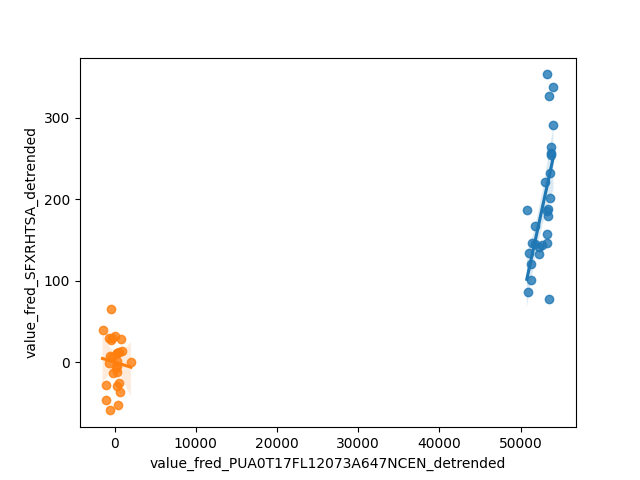
\includegraphics[scale = 0.9]{plots/plot_2026-10-30_detrended.png}
\caption{Detrended Regression Plot for 2026-10-30}
\end{figure}
\newpage
